%%%%%%%%%%%%%%%%%%%%%%%%%%%%%
%% Styles, packages and new commands
\input{../Main/ML_Main.tex}
%%%%%%%%%%%%%%%%%%%%%%%%%%%%%
%% Edit the title page
\title{Machine Learning}
\subtitle{Module 2: Data Exploration}
\author[MOB]{Marc-Olivier Boldi}
\institute[HEC MSc Mgt BA]{Master in Management, Business Analytics, HEC UNIL}
\date[Spring 2024]{Spring 2024}
%%%%%%%%%%%%%%%%%%%%%%%%%%%%%
%%%%%%%%%%%%%%%%%%%%%%%%%%%%%
%%%%%%%%%%%%%%%%%%%%%%%%%%%%%
%%%%%%%%%%%%%%%%%%%%%%%%%%%%%
\begin{document}
%%%%%%%%%%%%%%%%%%%%%%%%%%%%%
\begin{frame}
	\titlepage
\end{frame}
%%%%%%%%%%%%%%%%%%%%%%%%%%%%%
\begin{frame}
\frametitle{Table of Contents}
	\tableofcontents
\end{frame}
%%%%%%%%%%%%%%%%%%%%%%%%%%%%%
\section{Meta data}
%%%%%%%%%%%%%%%%%%%%%%%%%%%%%
\begin{frame}
\frametitle{Data set information}
{\bf Meta data} refers to information (data) about the data set itself. In data science, this usually includes
\begin{itemize}
\item Its origin and/or source, if possible, the first one (not only the web page from which it was retieved).
\item Its dates of creation and/or retrieval.
\item Its name and/or title.
\item Its file type (csv, xlxs, etc.).
\item Its shape and a general description of its content (each column for tabular data).
\end{itemize}
E.g., see {\tt ?bank} in the package {\tt liver}. 
\end{frame}
%%%%%%%%%%%%%%%%%%%%%%%%%%%%%
\section{Data Expolration}
%%%%%%%%%%%%%%%%%%%%%%%%%%%%%
\begin{frame}
\frametitle{EDA}
{\bf EDA} stands for Exploratory Data Analysis. It is {\bf not} optional! Aims:
\begin{itemize}
\item Know the data: e.g., number of modalities for categorical variables, data length, number of missing values, etc.
\item Be informed of their general behavior: modality proportions, location and dispersion of numerical variables, etc.
\item Detect any outliers or special modes.
\item Inspect some of the data relationships.
\end{itemize}
There exist endless possibilities of EDA. A range of classical and efficient methods is presented below.
\end{frame}
%%%%%%%%%%%%%%%%%%%%%%%%%%%%%
\begin{frame}
\frametitle{EDA strategy}
Without prior knowledge of the case:
\begin{itemize}
\item One by one: univariate analysis.
\item By pairs: bivariate analysis. 
\item More variables if needed and/or possible.
\end{itemize}
\end{frame}
%%%%%%%%%%%%%%%%%%%%%%%%%%%%%
\begin{frame}
\frametitle{Exploratory tools}
For univariate analysis (one variable):\\
\vspace{0.3cm}
Graphical:
\begin{itemize}
\item Categorical variables: barplot and stacked barplot
\item Numerical variables: boxplot, violin plot, and histogram.
\end{itemize}
Numerical:
\begin{itemize}
\item Categorical variables: frequencies and proportions,
\item Numerical variables: locations (mean, median, min, max), dispersions (standard deviation, IQR, range), quantiles ($0.25, 0.75$),
\item Both: number of observations, number of missing values.
\end{itemize}
\end{frame}
%%%%%%%%%%%%%%%%%%%%%%%%%%%%%
\begin{frame}
\frametitle{Exploratory tools}
For bivariate analysis (two variables):\\
\vspace{0.3cm}
Graphical:
\begin{itemize}
\item cat*cat: barplots, mosaic plots 
\item cat*num: boxplots or histograms of num per modality of cat 
\item num*num: scatterplot 
\end{itemize}
Numerical:
\begin{itemize}
\item cat*cat: table of frequencies or proportions
\item cat*num: statistics of num per modality of cat
\item num*num: correlation
\end{itemize}
\end{frame}
%%%%%%%%%%%%%%%%%%%%%%%%%%%%%
\begin{frame}
\frametitle{Exploratory tools}
For more than two variables this mainly depends on the objective. The complexity increases fast and no universal method exists. Consider
\begin{itemize}
\item cat*cat*cat: Sankey diagram.
\item num*num*num: parallel coordinates.
\item num*num*cat: scatterplot (num*num) with colors or shapes (cat).
\item cat*cat*num: can turn num into cat (intervals) or can make cat*cat = cat (combine modalities).
\end{itemize}
\end{frame}
%%%%%%%%%%%%%%%%%%%%%%%%%%%%%
\section{Data transformation}
%%%%%%%%%%%%%%%%%%%%%%%%%%%%%
\begin{frame}
\frametitle{Numerical variables}
Many possibilities. Consider,
\begin{itemize}
\item Univariate: $x^2$, $\ln(x)$, $\ln(1+x)$, $|x|$, $1/x$, ranks, etc.
\item Multivariate: $x_1 x_2$, $x_1 + x_2$, etc.
\item Num to ordinal: categorize $x$ by intervals.
\end{itemize}
Applying any transformation must be guided by the aim of the study (e.g., use $\ln(1+x)$ on the outcome $x\geq 0$). 
\end{frame}
%%%%%%%%%%%%%%%%%%%%%%%%%%%%%
\begin{frame}
\frametitle{Categorical variables}
Many possibilities. Consider,
\begin{itemize}
\item Turn ordinal into num (1, 2, 3, etc.).
\item Diminish the number of modalities if too many: e.g., A, B, C covers $80\%$ of the cases. Create a category "other" for the rest.
\item Create dummy variables.
\end{itemize}
\end{frame}
%%%%%%%%%%%%%%%%%%%%%%%%%%%%%
\begin{frame}
\frametitle{Dummy variables}
ML algorithms perform mathematical operations on the data. They require numbers and cannot be performed on categorical data (characters, strings, etc.). These are then represented as {\bf dummy variables}. \\
\vspace{0.3cm}
Most functions in {\tt R} handle these representations automatically. However, it is not always the case in {\tt Python} or in other computer programs. In any cases, it is important to know what is being the scene and how to represent categorical variables as dummy variables.
\end{frame}
%%%%%%%%%%%%%%%%%%%%%%%%%%%%%
\begin{frame}
\frametitle{Dummy variable}
Transform a categorical variable into several numerical variables:
\begin{itemize}
\item One modality is the {\bf reference} (choice of the user).
\item For the other modalities: $0/1$ variables, one per modality. 
\item Value is 1 if the modality is the same as the modality of the dummy variable, 0 otherwise.
\end{itemize}
Note: one variable, called {\bf intercept}\footnote{In most algorithm, especially in regressions. In Neural Network, it is called the {\bf bias}.}, made of 1's, is added.
\end{frame}
%%%%%%%%%%%%%%%%%%%%%%%%%%%%%
\begin{frame}
\frametitle{Dummy variable example}
A variable indicates a shape. It has three levels {\tt Cloud}, {\tt Moon}, and {\tt Star}. The reference level below is {\tt Cloud}. Below, 15 instances. 
\begin{center}
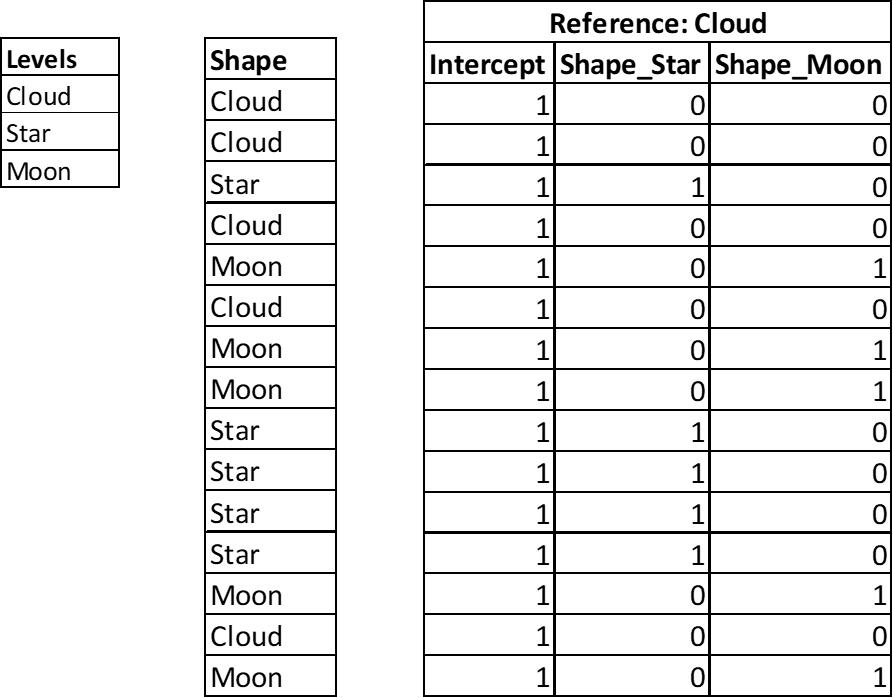
\includegraphics[width=8cm]{../Graphs/Dummy_1.png}  
\end{center}
\end{frame}
%%%%%%%%%%%%%%%%%%%%%%%%%%%%%
\begin{frame}
\frametitle{Dummy variable example}
The same example when the reference level below is {\tt Moon}. 
\begin{center}
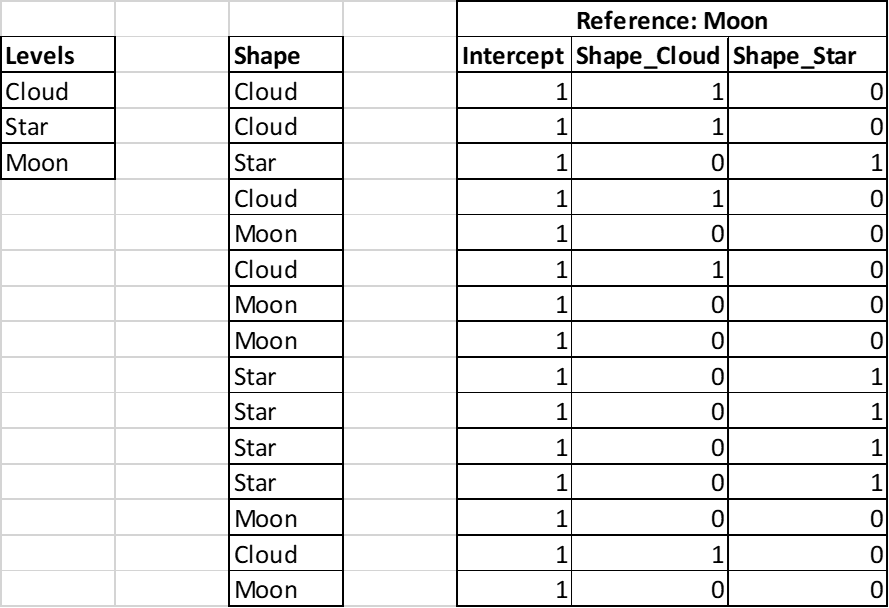
\includegraphics[width=8cm]{../Graphs/Dummy_2.png}  
\end{center}
\end{frame}
%%%%%%%%%%%%%%%%%%%%%%%%%%%%%
\section{Missing values}
%%%%%%%%%%%%%%%%%%%%%%%%%%%%%
\begin{frame}
\frametitle{Dealing with (without) missing values}
Missing value analysis is {\bf never} easy and would deserve a whole course. In a quick fix, consider
\begin{itemize}
\item Detect: which variables, which code (e.g., {\tt NA}, $-999$, etc.).  
\item Quantify: how many (number and proportion) for variables and cases.
\item Relate: two (or more) variables are systematically missing together?
\end{itemize}
In absence of data, lot of techniques break down. Can this be solved perfectly? No.
\end{frame}
%%%%%%%%%%%%%%%%%%%%%%%%%%%%%
\begin{frame}
\frametitle{Dealing with (without) missing values}
Various techniques, none of which is perfect:
\begin{itemize}
\item Remove the cases with at least one missing feature.
\item Remove the feature with too many missing values.
\item Input the missing value.
\end{itemize}
\end{frame}
%%%%%%%%%%%%%%%%%%%%%%%%%%%%%
\begin{frame}
\frametitle{Remove cases}
Pro:
\begin{itemize}
\item Very simple and systematic
\end{itemize}
Cons:
\begin{itemize}
\item Can leave no data: e.g., one variable is $99\%$ systematically missing.
\item Can bias the analysis: e.g., missing is linked to the outcome (NMAR)
\end{itemize}
\end{frame}
%%%%%%%%%%%%%%%%%%%%%%%%%%%%%
\begin{frame}
\frametitle{Remove features}
Pro:
\begin{itemize}
\item if most of the missing values are concentrated in one feature, then it saves lot of cases.
\end{itemize}
Cons:
\begin{itemize}
\item Can leave out important information.
\end{itemize}
Consider also replacing the feature by indicator "0/1" for missing or not. 
\end{frame}
%%%%%%%%%%%%%%%%%%%%%%%%%%%%%
\begin{frame}
\frametitle{Imputation}
\begin{itemize}
\item {\bf Naive:} per feature, replace NA by average or median (num), or the most frequent modality (cat). 
\begin{itemize}
\item Pro: None.
\item Cons: Avoid if possible (even if it is often used).
\end{itemize}
\item {\bf Model based:} use the other features to predict the missing one (case by case).
\begin{itemize}
\item Pro: Use all the available information.
\item Cons: Incorrectly diminish the noise in the data which enforce the correlation and give a wrong impression of certainty.
\end{itemize}
\end{itemize}
More advanced methods: repeated random imputation, EM algorithm, etc.
\end{frame}
%%%%%%%%%%%%%%%%%%%%%%%%%%%%%
\section{Outliers}
%%%%%%%%%%%%%%%%%%%%%%%%%%%%%
\begin{frame}
\frametitle{Definition}
Behind the term {\bf outlier} hides lots of ideas. It can be (non-exhaustive)
\begin{itemize}
\item An impossible value: exceeding physical limits.
\item An extreme value of a feature: possible but out of some predefined bounds. 
\item An unlikely value: unlikely given the other features.
\end{itemize}
The second case is limited to numerical features. The two others can be categorical features.
\end{frame}
%%%%%%%%%%%%%%%%%%%%%%%%%%%%%
\begin{frame}
\frametitle{Detection}
For the three previous cases, consider
\begin{itemize}
\item Often easy to detect from prior information. E.g., negative surface in a real estate data study, time exceeding 1 hour in a 1-hour observation study, etc. 
\item Use boxplot to point them: values beyond $1.5$ IQR from the quartile. E.g., age of 101 years when the other largest observed is 35 years.
\item Complex: use prior knowledge or a model. E.g., a room used for an RMI in a hospital for a specific diagnostic for which this room is never used, a yearly wage greater than $\$1'000'000$ for a job in manufacturing.
\end{itemize}
\end{frame}
%%%%%%%%%%%%%%%%%%%%%%%%%%%%%
\begin{frame}
\frametitle{Discussion}
With outliers, things are never simple and automatic removal is often a bad idea. In an ideal world, only errors should be removed. Consider,
\begin{itemize}
\item {\bf Check the facts}: how many (if only one then it could be removed safely), where, which features?
\item Inquiry {\bf how the data were gathered}: e.g., $5\%$ of the revenues are negative. Did you consider possible that the revenue could indeed be negative in that study?
\item If set aside then {\bf document it}. This should never be hidden.
\item In some situation, outliers are of interest: e.g., fraud analytics.
\end{itemize}
\end{frame}
%%%%%%%%%%%%%%%%%%%%%%%%%%%%%
\section{Further words}
%%%%%%%%%%%%%%%%%%%%%%%%%%%%%
\begin{frame}
\frametitle{Further words}
\begin{itemize}
\item Analyze all variables systematically (univariate).
\item Bivariate can be too complex. Select the intersting ones (e.g., in supervised learning, outcome vs other).
\item Multivariate analysis be selective.
\end{itemize}
Common fallacies:
\begin{itemize}
\item Use too many modalities in a categorical variable.
\item Compute correlations between dummy variables.
\item Use missing value indicator as a number (e.g., -999).
\item Transformations are not neutral. They influence the final conclusion. They must be taken into account and transparent.
\item Think that EDA is a one way through. It is a recursive/trial-and-error process (not unusual $90\%$ of the work...)
\end{itemize}
\end{frame}
%%%%%%%%%%%%%%%%%%%%%%%%%%%%%
\end{document}
%%%%%%%%%%%%%%%%%%%%%%%%%%%%%

\begin{frame}
\frametitle{Further words}
There exist lots of other possibilities and modifications of the previous examples. EDA is a {\bf crucial} part of the analysis. It allows to have a first contact with the data, to identify possible issues or peculiarities. It motivates any decision to
\begin{itemize}
\item modify, increase the data (feature engineering, merging levels, recoding the data, etc.),
\item control data quality (number of levels due to bad coding, missing values, outliers, etc.),
\item look for better understanding of data (check definition, source, extraction process, etc.),
\item check for association between variables and anticipate the model results.
\end{itemize}
\end{frame}
%%%%%%%%%%%%%%%%%%%%%%%%%%%%%

\begin{frame}
\frametitle{Cat - Cat}
Crossing two categorical variables: barplots 
\begin{center}
\includegraphics[width=8cm]{../Graphs/imports85_barplots.png}
\end{center}
\end{frame}
%%%%%%%%%%%%%%%%%%%%%%%%%%%%%
\begin{frame}
\frametitle{Num - Num}
Crossing two numerical variables: scatterplots 
\begin{center}
\includegraphics[width=8cm]{../Graphs/imports85_scatterplot.png}
\end{center}
\end{frame}
%%%%%%%%%%%%%%%%%%%%%%%%%%%%%
\begin{frame}
\frametitle{Num - Cat}
Crossing one numerical and one categorical variable: boxplots 
\begin{center}
\includegraphics[width=8cm]{../Graphs/imports85_boxplots.png}
\end{center}
\end{frame}
%%%%%%%%%%%%%%%%%%%%%%%%%%%%%
\section{Data transformation}
%%%%%%%%%%%%%%%%%%%%%%%%%%%%%
\begin{frame}
\frametitle{General}
Several data transformations can be useful:
\begin{itemize}
\item Coding categorical variables: dummy variables for nominal data, numerical rank for ordinal data.
\item Transformation of numerical variables: functions like $\log(x)$, $\exp(x)$, $x^2$. 
\item Recoding categorical variables: e.g., merge the smallest classes as ``others''.
\item Recoding numerical variable: value to interval to ordinal data.
\item Interaction: combine several variables.
\end{itemize} 
Often referred to as {\bf feature engineering}.
\end{frame}
%%%%%%%%%%%%%%%%%%%%%%%%%%%%%
\begin{frame}
\frametitle{Dummy variables}
ML algorithms perform mathematical operations on the data. They require numbers and cannot be performed on categorical data (characters, strings, etc.). These are then represented as {\bf dummy variables}. \\
\vspace{0.3cm}
Most functions in {\tt R} handle these representations automatically. However, it is not always the case in {\tt Python} or in other computer programs. In any cases, it is important to know what is being the scene and how to represent categorical variables as dummy variables.
\end{frame}
%%%%%%%%%%%%%%%%%%%%%%%%%%%%%
\begin{frame}
\frametitle{Dummy variable}
\begin{itemize}
\item A categorical variables has a given number of possible values called {\bf levels}.
\item One level is taken as the {\bf reference}. This is arbitrary (choice of the user).
\item The dummy variables consist in a set of 0/1 valued variables, one per levels {\bf that are not the reference level}. 
\item The value of each dummy variable is 1 if the categorical variable value is the same as the level of the dummy variable, 0 otherwise.
\item One variable, called {\bf intercept}\footnote{In most algorithm, especially in regressions. In Neural Network, it is called the {\bf bias}.}, made of 1's, is added.
\end{itemize}
\end{frame}
%%%%%%%%%%%%%%%%%%%%%%%%%%%%%
\begin{frame}
\frametitle{One variable example}
A variable indicates a shape. It has three levels {\tt Cloud}, {\tt Moon}, and {\tt Star}. The reference level below is {\tt Cloud}. Below, 15 instances. 
\begin{center}
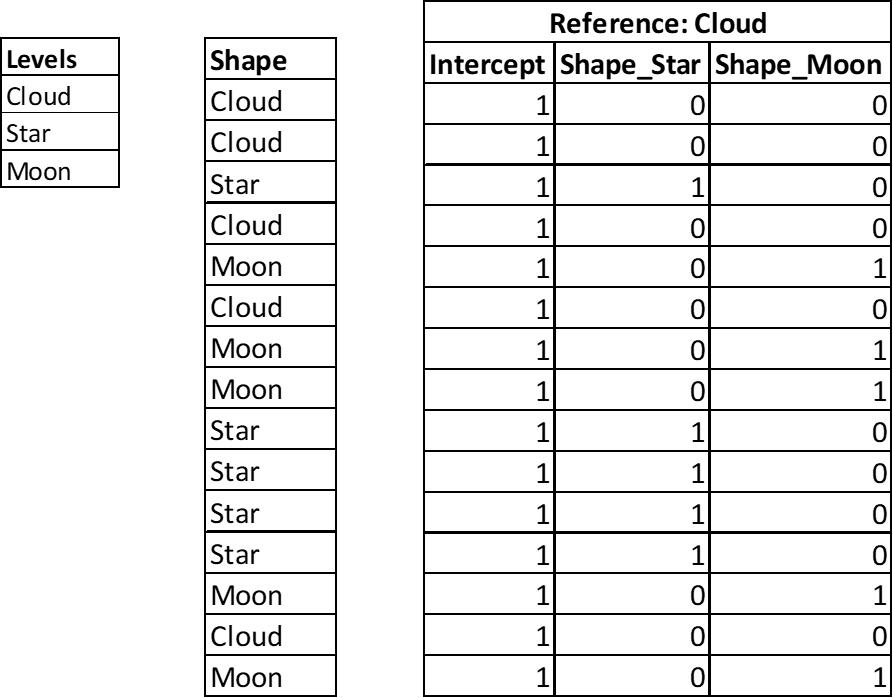
\includegraphics[width=8cm]{../Graphs/Dummy_1.png}  
\end{center}
\end{frame}
%%%%%%%%%%%%%%%%%%%%%%%%%%%%%
\begin{frame}
\frametitle{One variable example}
The same example when the reference level below is {\tt Moon}. 
\begin{center}
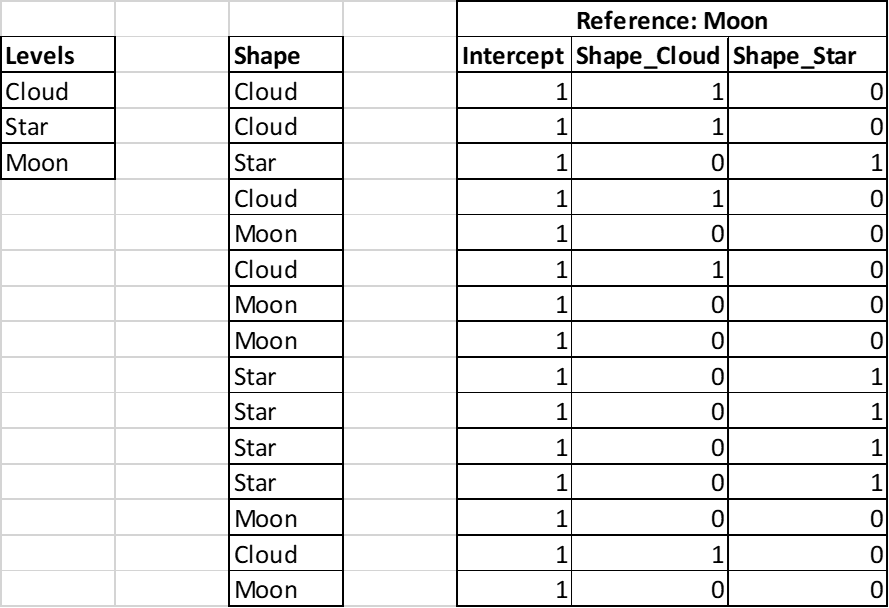
\includegraphics[width=8cm]{../Graphs/Dummy_2.png}  
\end{center}
\end{frame}
%%%%%%%%%%%%%%%%%%%%%%%%%%%%%
\begin{frame}
\frametitle{More than one variable}
When there are several categorical variables,
\begin{itemize}
\item There is one set of dummy variables per categorical variables.
\item Obviously, each categorical variable has its reference level.
\item There is only one intercept variable (for all the categorical variables).
\end{itemize}
\end{frame}
%%%%%%%%%%%%%%%%%%%%%%%%%%%%%
\begin{frame}
\frametitle{More than one variable}
Below the example with two categorical variables:
\begin{center}
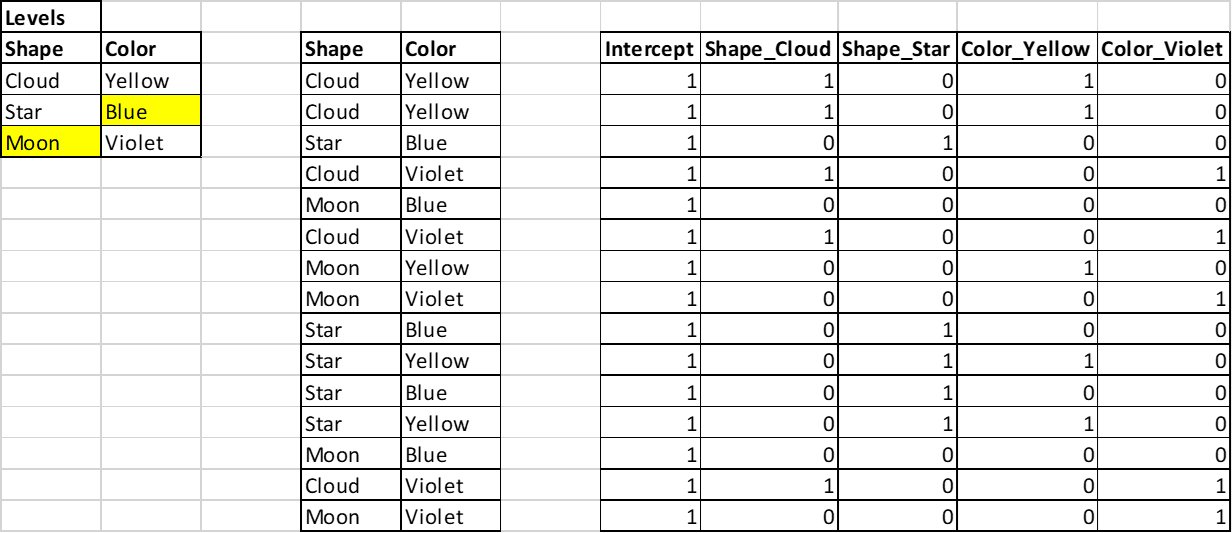
\includegraphics[width=10cm]{../Graphs/Dummy_3.png}  
\end{center}
\scriptsize
Notes: there could have been more than three levels each time. The reference levels are indicated in yellow.
\normalsize
\end{frame}
%%%%%%%%%%%%%%%%%%%%%%%%%%%%%
\begin{frame}
\frametitle{Why an intercept?}
Having an intercept is the most efficient\footnote{There exist several ways to code categorical variables into dummy variables but they all define reference levels and an intercept of some sort.} way of coding several categorical variables. Keeping all the dummy, like in the example below, impose to carry more columns in the data set, that is {\it redundant information}. We do not want that.
\begin{center}
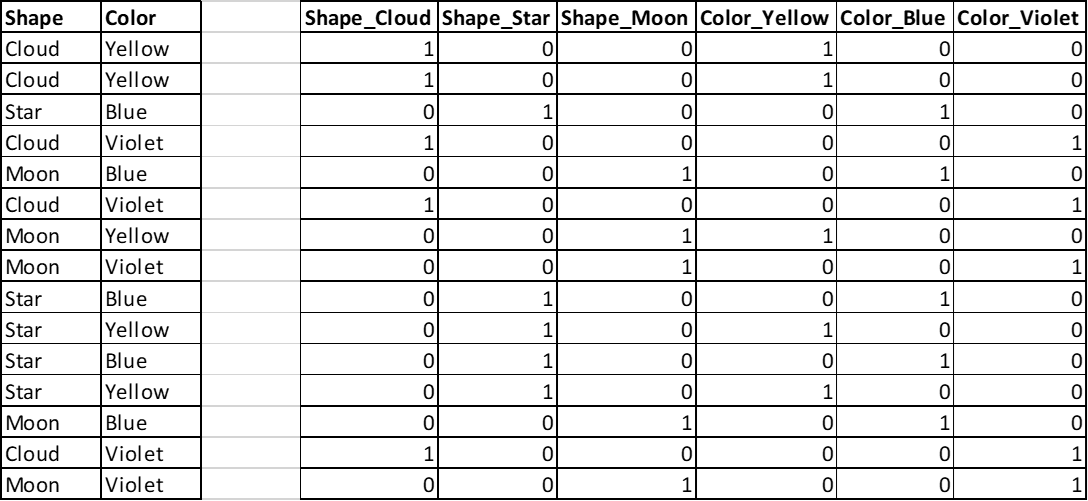
\includegraphics[width=10cm]{../Graphs/Dummy_4.png}  
\end{center}
\end{frame}
%%%%%%%%%%%%%%%%%%%%%%%%%%%%%
\begin{frame}
\frametitle{Number of columns and levels}
\begin{itemize}
\item The number of columns in the data set depends on the number of levels. Thus, it cannot be known in advance if the data itself is not known. In practice, one cannot add levels to a categorical variable without handling a new analysis/model training. 
\item If there are $J$ categorical variables, each with $n_j$ levels, the number of columns will be
$$
1 + \sum_{j=1}^J (n_j - 1)
$$
That number can grow very quickly with either the number of variables and the number of levels. 
\end{itemize}
\end{frame}
%%%%%%%%%%%%%%%%%%%%%%%%%%%%%
\begin{frame}
\frametitle{Transformation of numerical variables}
In practice, it can be a good idea to
\begin{itemize}
\item transform some of the existing variables,
\item add newly created one.
\end{itemize}
Any mathematical transformation can be tried and is, a priori, justified: $\log(x)$, $\exp(x)$, $\sqrt{x}$, $x^p$, etc.
\end{frame}
%%%%%%%%%%%%%%%%%%%%%%%%%%%%%
\begin{frame}[fragile]
\frametitle{Transformation of numerical variables}
For example, the iris data set is a  famous data set linking the flower species (Virginica, Setosa, Versicolor) to the flower dimensions (petal and sepal, length and width). It contains 150 instances. It is a playground for testing/developing classification techniques.\\
\scriptsize
\begin{verbatim}
> head(iris)
  Sepal.Length Sepal.Width Petal.Length Petal.Width Species
1          5.1         3.5          1.4         0.2  setosa
2          4.9         3.0          1.4         0.2  setosa
3          4.7         3.2          1.3         0.2  setosa
4          4.6         3.1          1.5         0.2  setosa
5          5.0         3.6          1.4         0.2  setosa
6          5.4         3.9          1.7         0.4  setosa
\end{verbatim}
\normalsize
\end{frame}
%%%%%%%%%%%%%%%%%%%%%%%%%%%%%
\begin{frame}
\frametitle{Transformation of numerical variables}
From two iris data features (sepal length and width), two new features were created: square of the length and logarithm of the width.
\begin{center}
\includegraphics[width=9cm]{../Graphs/FeatEng.png}
\end{center}
\end{frame}
%%%%%%%%%%%%%%%%%%%%%%%%%%%%%
\begin{frame}
\frametitle{Good practice}
When feature engineering comes into play, there is no limit a priori since one can create an infinite number of features. Some good practices are:
\begin{itemize}
\item adding variables like $-x$ or any linear transformation $a+bx$ is often useless.
\item Use $\log(x)$, $\sqrt{x}$ only on positive variables, or consider applying them on $1+x$.
\item The interest of $\log$ or any power $0<p<1$ (like $\sqrt{x}$) is to ``de-concentrate'' the data.
\item The interest of $\exp$ is to expand the data.
\item The interest of $x^2$ or $|x|$ is to see the effect of removing the sign of the variable value.
\item New features {\bf must} never include the outcome in any way. 
\end{itemize}
\end{frame}
%%%%%%%%%%%%%%%%%%%%%%%%%%%%%
\begin{frame}
\frametitle{Recoding categorical variables}
We often consider two types of possible recoding:
\begin{itemize}
\item Diminishing the number of levels. Especially when several levels have very low frequencies in the data set and when these levels are {\bf not} of specific interest, then merging these levels into a common one (e.g., ``Other'') may balance the data and improve the analysis.
\item Coding an ordinal variable into a Liker scale. For example, XS/S/M/L/XL may be coded to (numbers) $1, 2, 3, 4, 5$. This is not equivalent to using dummy variables but may even improve the analysis and make it more interpretable. However, it is {\bf not} a good idea with a nominal variable.
\end{itemize}
\end{frame}
%%%%%%%%%%%%%%%%%%%%%%%%%%%%%
\begin{frame}
\frametitle{Recoding numerical variables}
In some cases, especially when it makes sense in the context, it may be a good idea to build {\bf interval data} from a numerical one. This is typical for revenue data, time data, etc.\\
\vspace{0.3cm}
For example, a percentage data may be turned into an ordinal variable with five levels $[0,0.2], ]0.2,0.4], ]0.4,0.6], ]0.6,0.8], ]0.8,1]$. \\
\vspace{0.3cm}
The number of intervals and their shape (regular or not) should make sense in the context and there is no general rule. In practice however, one would avoid to build empty interval (i.e. without any observation in it).
\end{frame}
%%%%%%%%%%%%%%%%%%%%%%%%%%%%%
%\section{Interactions}
%%%%%%%%%%%%%%%%%%%%%%%%%%%%%
\begin{frame}
\frametitle{Interactions}
{\bf Interactions}, especially in the context of regression models (linear regression, logistic regression, etc.), refer to the multiplication between two variables
\begin{itemize}
\item Between two numerical features, $x_1x_2$.
\item Between one numerical and one categorical variables: multiply the numerical and the dummy variables.
\item Between two categorical variables: multiply all the dummy variables across the two categorical variables ({\it not} the dummy variables from the same categorical variable!).
\end{itemize}
\end{frame}
%%%%%%%%%%%%%%%%%%%%%%%%%%%%%
\begin{frame}
\frametitle{Interactions}
Example mixing the shape/color data and the iris data.
\begin{center}
\includegraphics[width=9cm]{../Graphs/Interaction_1.png}
\end{center}
\end{frame}
%%%%%%%%%%%%%%%%%%%%%%%%%%%%%
\begin{frame}
\frametitle{Interactions}
Example with the interactions between shape and color:
\begin{center}
\includegraphics[width=9cm]{../Graphs/Interaction_2.png}
\end{center}
\end{frame}
%%%%%%%%%%%%%%%%%%%%%%%%%%%%%
\begin{frame}
\frametitle{Discussion}
\begin{itemize}
\item The number of columns in the data set can expand very quickly. 
\item One can also consider three-way interactions (based on $x_1x_2x_3$) or higher-order interaction terms. 
\item Once being defined, interactions can be treated like any other features and further transformation can be applied to them. 
\item More generally, feature engineering also includes combinations like $\log(x_1x_2+1)$, $\exp(x_1/x_2)$, etc.
\end{itemize}
\end{frame}
%%%%%%%%%%%%%%%%%%%%%%%%%%%%%

\begin{frame}
\frametitle{Structure}
{\tt imports.85}: a data frame of characteristics of cars. let's see its structure. 
\begin{center}
\includegraphics[width=7cm]{../Graphs/imports85_structure.png}
\includegraphics[width=7cm]{../Graphs/imports85_head.png}
\end{center}
\end{frame}
%%%%%%%%%%%%%%%%%%%%%%%%%%%%%
\begin{frame}
\frametitle{Global summary}
The default summary function.
\begin{center}
\includegraphics[width=8cm]{../Graphs/imports85_summary.png}
\end{center}
\end{frame}
%%%%%%%%%%%%%%%%%%%%%%%%%%%%%
\begin{frame}
\frametitle{Global summary (2)}
A more fancy one.
\begin{center}
\includegraphics[width=9cm]{../Graphs/imports85_dfsummary.png}
\end{center}
\end{frame}
%%%%%%%%%%%%%%%%%%%%%%%%%%%%%
\begin{frame}
\frametitle{Categorical variables}
Pie chart for one of the categorical variables ({\tt make})
\begin{center}
\includegraphics[width=13cm]{../Graphs/imports85_piechart.png}
\end{center}
\end{frame}
%%%%%%%%%%%%%%%%%%%%%%%%%%%%%
\begin{frame}
\frametitle{Categorical variables}
Barplot
\begin{center}
\includegraphics[width=9cm]{../Graphs/imports85_onebarplot.png}
\end{center}
\end{frame}
%%%%%%%%%%%%%%%%%%%%%%%%%%%%%
\begin{frame}
\frametitle{Categorical variables}
Stacked barplot
\begin{center}
\includegraphics[width=8cm]{../Graphs/imports85_stackedbarplot.png}
\end{center}
\end{frame}
%%%%%%%%%%%%%%%%%%%%%%%%%%%%%
\begin{frame}
\frametitle{Numerical variables}
Boxplot for one of the numerical variables ({\tt price})
\begin{center}
\includegraphics[width=6cm]{../Graphs/imports85_oneboxplot.png}
\end{center}
\end{frame}
%%%%%%%%%%%%%%%%%%%%%%%%%%%%%
%\begin{frame}
%\frametitle{Numerical variables}
%Violin plot
%\begin{center}
%\includegraphics[width=6cm]{../Graphs/imports85_violinplot.png}
%\end{center}
%\end{frame}
%%%%%%%%%%%%%%%%%%%%%%%%%%%%%
\begin{frame}
\frametitle{Numerical variables}
Histogram
\begin{center}
\includegraphics[width=8cm]{../Graphs/imports85_histogram.png}
\end{center}
\end{frame}
\begin{frame}
\frametitle{More than one variable}
When there are several categorical variables,
\begin{itemize}
\item There is one set of dummy variables per categorical variables.
\item Obviously, each categorical variable has its reference level.
\item There is only one intercept variable (for all the categorical variables).
\end{itemize}
\end{frame}
%%%%%%%%%%%%%%%%%%%%%%%%%%%%%
\begin{frame}
\frametitle{More than one variable}
Below the example with two categorical variables:
\begin{center}
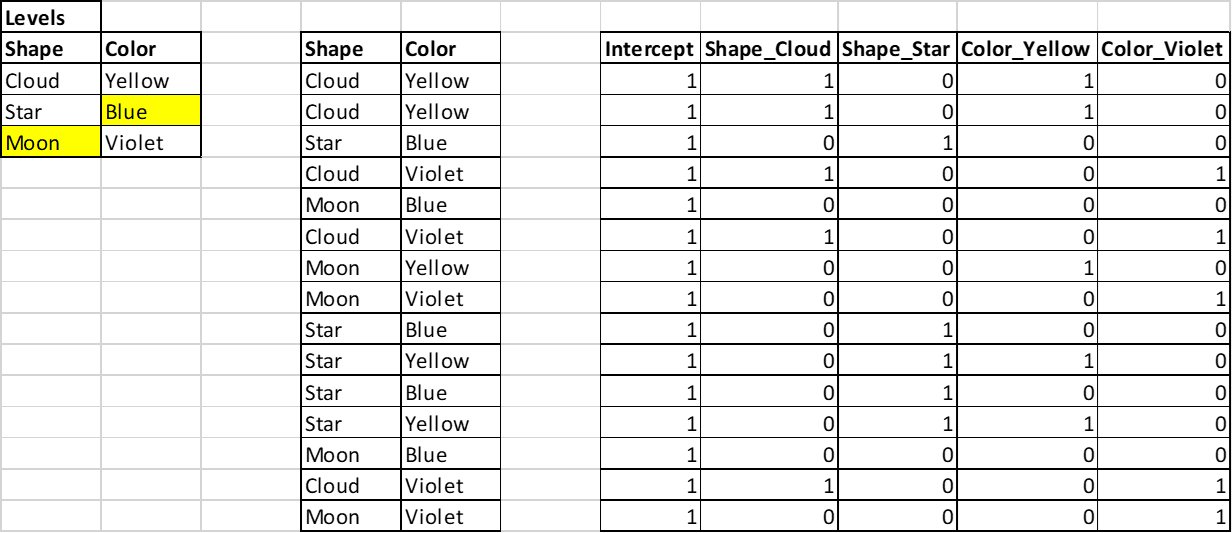
\includegraphics[width=10cm]{../Graphs/Dummy_3.png}  
\end{center}
\scriptsize
Notes: there could have been more than three levels each time. The reference levels are indicated in yellow.
\normalsize
\end{frame}
%%%%%%%%%%%%%%%%%%%%%%%%%%%%%
\begin{frame}
\frametitle{Why an intercept?}
Having an intercept is the most efficient\footnote{There exist several ways to code categorical variables into dummy variables but they all define reference levels and an intercept of some sort.} way of coding several categorical variables. Keeping all the dummy, like in the example below, impose to carry more columns in the data set, that is {\it redundant information}. We do not want that.
\begin{center}
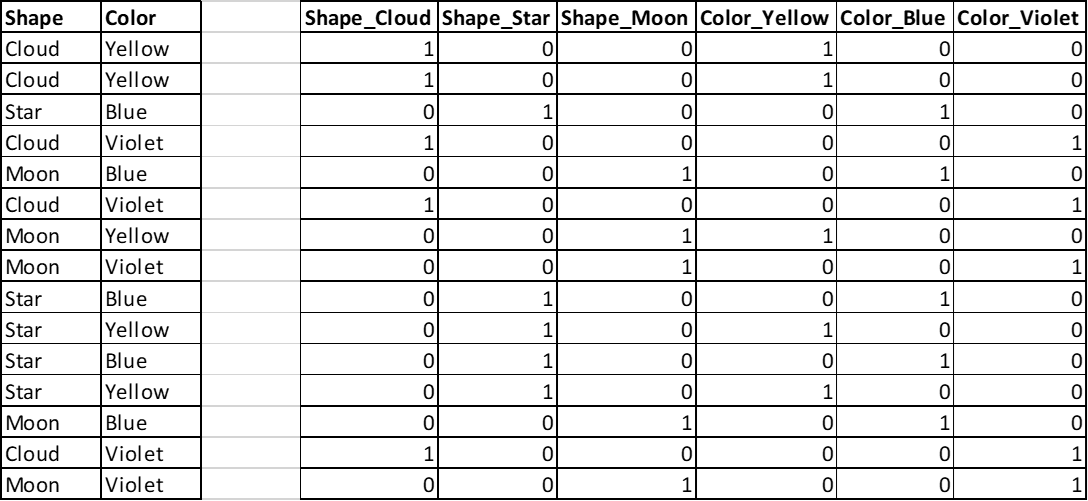
\includegraphics[width=10cm]{../Graphs/Dummy_4.png}  
\end{center}
\end{frame}
%%%%%%%%%%%%%%%%%%%%%%%%%%%%%
\begin{frame}
\frametitle{Number of columns and levels}
\begin{itemize}
\item The number of columns in the data set depends on the number of levels. Thus, it cannot be known in advance if the data itself is not known. In practice, one cannot add levels to a categorical variable without handling a new analysis/model training. 
\item If there are $J$ categorical variables, each with $n_j$ levels, the number of columns will be
$$
1 + \sum_{j=1}^J (n_j - 1)
$$
That number can grow very quickly with either the number of variables and the number of levels. 
\end{itemize}
\end{frame}
%%%%%%%%%%%%%%%%%%%%%%%%%%%%%
